\documentclass[11pt,a4paper]{article}
\usepackage{a4wide}
\usepackage{graphicx}
\usepackage{epsfig}
\usepackage{amsmath}
\usepackage{amsfonts}
\usepackage{amssymb}
\usepackage{ngerman}
\usepackage[T1]{fontenc}
\usepackage[utf8]{inputenc}
\inputencoding{latin1}
\usepackage{multirow}
\usepackage{hyperref}
\usepackage{float}
\usepackage{url}
\usepackage{csvsimple}
\usepackage{caption} 

\begin{document}
\Large\textbf{{{\noindent �bungsblatt 4 - Hochleistungsrechnen\\}}}
\textbf{{Leistungsanalyse\\}}
Tim Kilian, Joscha Fregin, Stefan Knispel
\section{Umsetzung der Datenaufteilungen}
Vergleich durchgef�hrt mit: partdiff-(spalten,zeilen,element) 12 2 512 2 2 1100\\
Element(static, 1):64.94s \\
Element (ohne scheduling): 57.37s\\
Zeilen: 65.25s \\
Spalten: 132.80s \\

Die elementweise Aufteilung l�uft am schnellsten. Wenn die Zerlegung der Matrix nicht festgelegt wird (kein scheduling) wird es noch schneller. Die Spaltenweise Aufteilung ist am langsamsten, weil durch das Vertauschen der Indices, der Speicher f�r den Programmablauf ung�nstig eingelesen wird. Dies ist bei der Zeilenmethode nicht der Fall, weshalb sie schneller ist (wie bei der ersten Optimierungsaufgabe zum sequentiellen Verfahren).




\section{Vergleich der Scheduling Algorithmen}
Der Vergleich der Algorithmen wurde auf dem Rechenknoten west7 durchgef�hrt mit folgenden Einstellungen: \\
./partdiff-openmp 12 2 512 2 2 1100, der code des sequentiellen Programms wurde nur durch die OpenMP Parallelisierung erweitert (keine Zeilen, Spalten Elementweise Aufteilung). Datenaufteilung durch Elemente wird sp�ter betrachtet.\\
Wie Tabelle \ref{tab1} zu entnehmen ist nicht ganz eindeutig welcher Algorithmus am besten funktioniert. 
guided l�uft zwar mit 48.85s am schnellsten, ist jedoch nicht so konstant wie die kaum langsamer laufende Einstellung dynamic (1,4). Am langsamsten l�uft der static Algorithmus. Er weist auch die gr��ten Schwankungen der Laufzeiten auf.

\begin{table}[h]
\centering
\begin{tabular}{ l|l|l|l }
   Blockgr. & dynamic & static & guided \\ \hline
     & 		 &  & 52.65 \\ 
     &		 & 	 &48.85  \\ 
     & 		&  	 & 49.05 \\ \hline
  1 & 49.46	 & 52.76 		 &  \\ 
     & 49.54	 & 61.74		 &  \\ 
    & 49.35	 	&  58.04		 & \\ \hline
  2 &  & 59.89 &  \\ 
      &  & 68.84 &  \\ 
         &  & 57.93 &  \\ \hline
   4 & 49.47 & 52.43 &  \\ 
    & 49.45 & 63.69 &  \\ 
     & 49.29 & 60.72 &  \\ \hline
     16 &  & 64.74 &  \\
         &  & 64.55 &  \\
                 &  & 62.74 &  \\ \hline

\end{tabular}
\caption{Vergleich der Scheduling Algorithmen mit jeweils drei Messl�ufen pro Einstellung in Sekunden}
\label{tab1}
\end{table}

\begin{table}[h]
\centering
\begin{tabular}{ l|l|l|l }
   Blockgr. & dynamic & static & guided \\ \hline
   & 	 	&  		 & 49.76 \\ \hline
   1 & 84.87	 	&  64.94		 & \\ \hline

      2   &  & 71.41 &  \\ \hline

     4& 59.35 & 56.18 &  \\ \hline

                16 &  & 66.79 &  \\ \hline

\end{tabular}
\caption{Vergleich der Scheduling Algorithmen f�r Elementzerlegung mit jeweils einem Messlauf pro Einstellung in Sekunden}
\label{tab2}
\end{table}
F�r die elementweise Zerlegung ist die guided Methode ebenfalls die schnellste. Jedoch ist dynamic langsamer als static (selbst bei gleicher Blockgr��e).


\section{Messung 1}

Bei der Messung 1 wurden die Parameter wie folgt gew�hlt:
- Threadanzahl ansteigend von 1 bis 12 \\
- Jacobi-Methode \\
- Interlines 512 \\
- St�rfunktion 2 \\
- 1100 Iterationen \\
Es wurde auf dem Rechnerknoten west5 gerechnet!
\noindent In der Abbildung \ref{messung1} ist die Berechnungszeit gegen die Anzahl der verwendeten Threads dargestellt. Die Berechnungszeit f�r einen einzelnen Thread dauert erwartungsgem�� am l�ngsten. Bei zwei verwendeten Threads halbiert sich die Berechnungszeit n�herungsweise. 
Plottet man die Berechnungszeit gegen�ber der Anzahl der Threads erh�lt man einen exponentiellen Verlauf. Hier ist deutlich zu erkennen, dass ab einer Verwendung von 6 Threads der Gradient sehr gering ist. Man erh�lt keine deutliche Verbesserung in der Berechnungszeit mehr im Vergleich zur Anzahl an Threads. 
Bei der Verwendung von 12 Threads verk�rzt sich die Berechnungszeit im Vergleich zu der mit einem Thread bei uns um den Faktor 11.5. Damit liegen wir innerhalb des geforderten Bereiches. \\
Das sequentielle Programm hat auf Knoten 7 581.856389 s (582.753409 s im zweiten Durchlauf) ben�tigt und liegt damit knapp �ber dem OpenMP Programm mit einem Thread. M�glicherweise funktiniert die Compileroptimierung f�r OpenMP hier besser, oder der Unterschied ist durch den Rechenknoten entstanden.

\begin{figure}[htb]
\centering
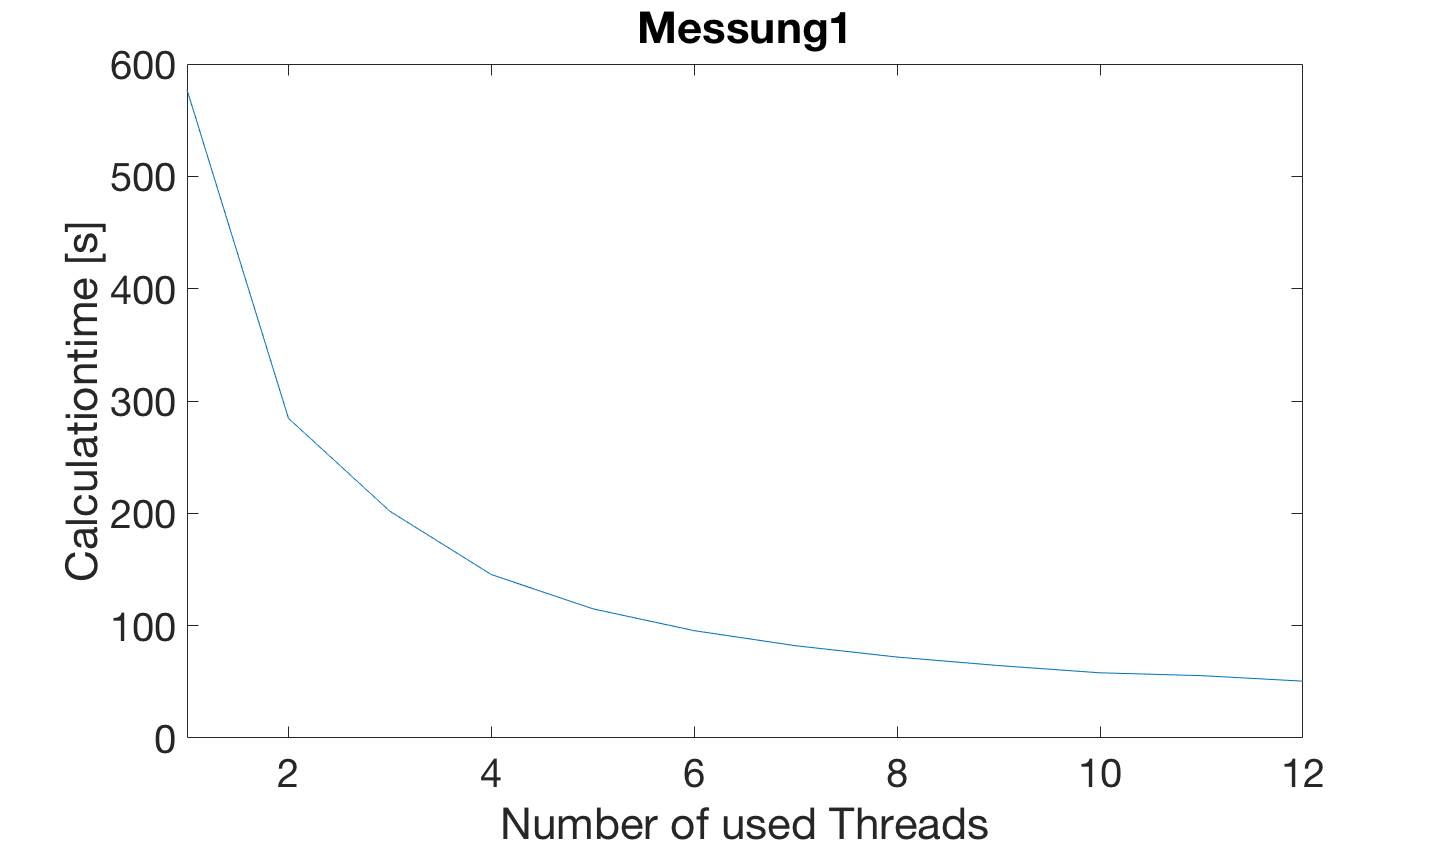
\includegraphics[width=1.0\textwidth,angle=0]{Messung1.png}
\caption{Messung 1 mit 512 Interlines und 1100 Iterationen.}
\label{messung1}
\end{figure}



\section{Messung 2}
Es wurde auf dem Rechnerknoten west5 gerechnet!
In der Abbildung \ref{messung2} ist die Berechnungszeit gegen die Anzahl der Interlines dargestellt. Es ist nicht eindeutig zu erkennen, ob hier ein exponentieller Verlauf vorliegt. Dazu m�sste mit noch weiteren Interlines gerechnet werden. Jedoch ist bei einer Anzahl von 1,2 oder 4 Interlines kein Unterschied in der Berechnungszeit zu erkennen. Jeder Durchlauf brachte Berechnungszeiten zwischen 0.3 und 0.9 Sekunden zum Vorschein. Das kommt durch die zu klein gew�hlte Matrix. Bei einer Zeilenanzahl von maximal 4 kann nicht jeder Thread eine Zeile zum Berechnen �bernehmen. Die Berechnungszeit m�sste theoretisch zwischen 1 und 12 Interlines fast identisch sein. Ab einer Interlines Anzahl von 13 m�sste diese erst wieder ansteigen, da dann mehr Zeilen als Threads vorhanden sind. \\

\begin{figure}[htb]
\centering
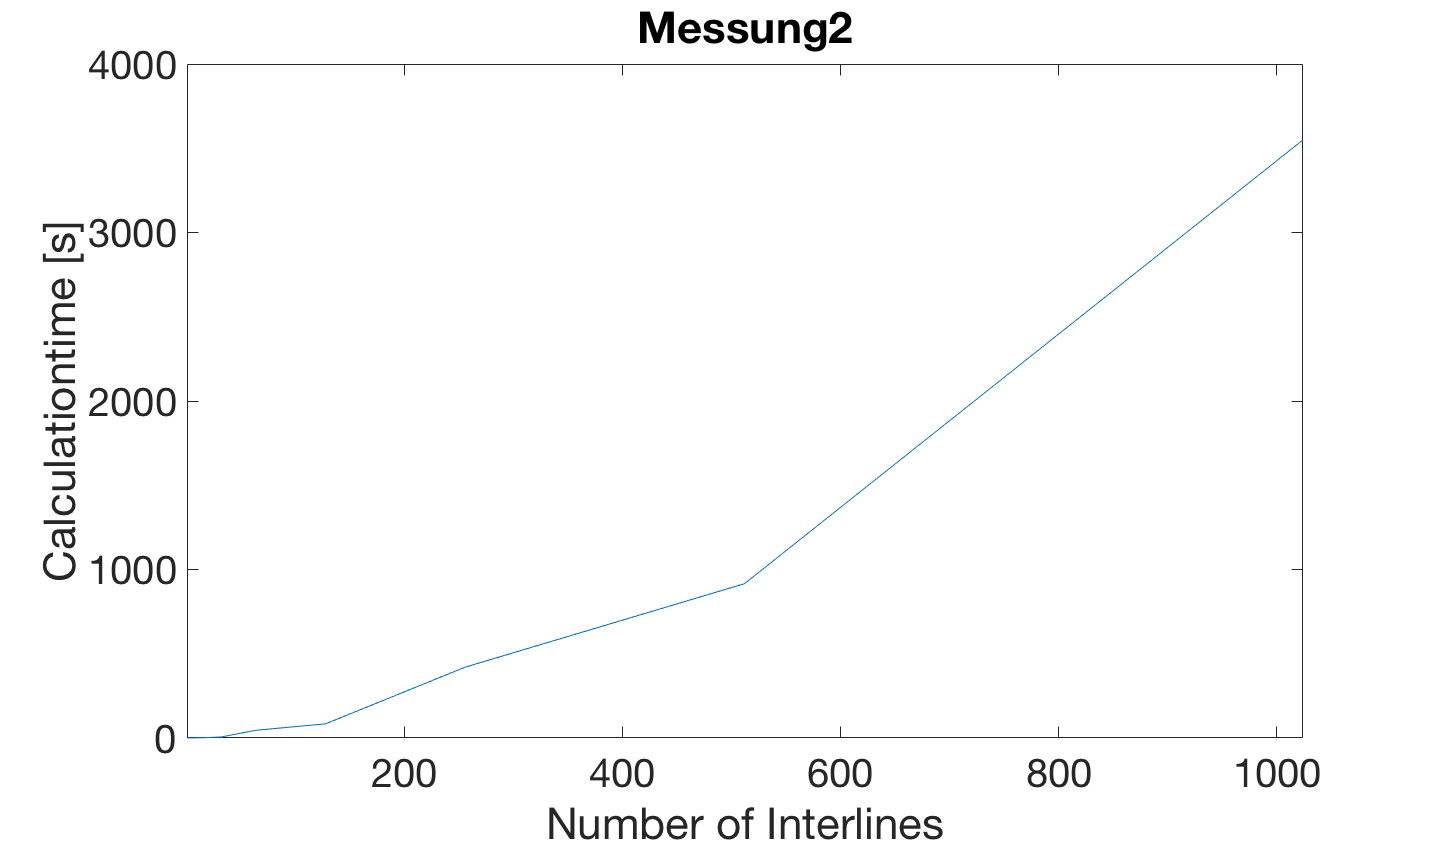
\includegraphics[width=1.0\textwidth,angle=0]{Messung2.png}
\caption{Messung 2 mit 20000 Iterationen und 12 Threads.}
\label{messung2}
\end{figure}



\end{document}